\documentclass{article}

% Packages
\usepackage[english]{babel}
\usepackage[a4paper,top=2cm,bottom=2cm,left=2.5cm,right=2.5cm,marginparwidth=1.75cm]{geometry}
\usepackage{amsmath}
\usepackage{graphicx}
\usepackage[colorlinks=true, allcolors=blue]{hyperref}
\usepackage{minted}
\usepackage{siunitx}
\usepackage{subcaption}

\title{Your Paper}
\author{You}

\begin{document}
\maketitle

\begin{abstract}
Your abstract.
\end{abstract}

\tableofcontents
%\newpage

\section{Basic Concepts}
%TODO check the implementation of the jet stream is correct with regards to the geostrophic relative vorticity calculation
For readers who are not familiar with atmospheric science, but who are familiar with Applied Mathematics, a brief overview of terminology and atmospheric properties is given.

\subsection{Layers of the Atmosphere}
The atmosphere is divided into a number of distinct layers, a characteristic referred to as \textit{stratification}. We will focus on the two layers closest to the Earth's surface: the troposphere and the stratosphere. The boundary between these two layers is known as the \textit{tropopause} \cite{Vallis2017}.

\begin{itemize}
    \item The \textbf{troposphere} extends from the Earth's surface ($z=0$) up to the tropopause. This layer is mostly transparent to incoming solar (shortwave) radiation, meaning it is primarily heated from below by terrestrial (longwave) radiation emitted by the Earth's surface. This bottom-up heating results in a negative vertical temperature gradient ($\frac{\partial T}{\partial z} < 0$) \cite{Vallis2017}. As a practical example, as you climb higher up a mountain, the temperature decreases with increasing altitude. The warmer air close to the surface is less dense than the colder air at higher altitudes, which leads to convective instability \cite{danielson2003meteorology}. Consequently, this layer experiences high turbulence \cite{sprenger2007userguide} and substantial dissipation of energy; almost all typical weather phenomena occur here.

    \item Above the troposphere lies the \textbf{stratosphere}. This layer contains a higher concentration of ozone, which absorbs high-energy ultraviolet (UV) solar radiation, heating the layer from within. Solar radiation first heats the ozone at higher altitudes, losing energy as it penetrates deeper into the lower stratosphere. This results in a positive temperature gradient ($\frac{\partial T}{\partial z} > 0$) \cite{Vallis2017}. Because warmer, less dense air sits atop cooler, denser air, the stratosphere is highly stable with respect to vertical convection \cite{Barnes2022main}.

    \item The \textbf{tropopause} serves as the boundary between the negative temperature gradient of the troposphere and the positive temperature gradient of the stratosphere. At this boundary, the temperature gradient experiences a discontinuity \cite{Panchev1985-et}. The altitude of the tropopause primarily varies with latitude ($\varphi$), occurring at an altitude of about \qty{16}{\km} in equatorial regions and dropping to approximately \qty{8}{\km} in polar regions \cite{Vallis2017}.
\end{itemize}

\subsection{Terminology}
The meaning of certain relevant terms that will be used later on is given. We assume that the reader is familiar with the quantities temperature ($T$), pressure ($p$), density ($\rho$) and acceleration due to gravity ($g$).

\begin{itemize}
    \item An \textbf{adiabatic} process is where a system exchanges no heat with its surroundings. In the case of the movement of an air parcel, the process is adiabatic if temperature only changes due to changes in pressure \cite{Vallis2017}.

    \item The \textbf{specific gas constant for dry air} ($R$) is \qty{287.05}{\joule\per\kg\per\kelvin}. It is used to relate $p$, $\rho$ and $T$ using the ideal gas law $p=\rho RT$ \cite{Vallis2017}.

    \item The \textbf{specific heat capacity of dry air} ($c_p$) is the amount of heat necessary to heat up \qty{1}{\kg} of dry air by \qty{1}{\kelvin}. We will take it to be \qty{1005}{\joule\per\kg\per\kelvin}

    \item \textbf{Potential temperature} ($\theta$) is the temperature an air parcel would attain if it were brought adiabatically to some reference pressure $p_0$. $p_0$ is usually taken to be \qty{1000}{\hecto\pascal} \cite{sprenger2007userguide}. \begin{equation}\label{pot_temp}
        \theta = T \left( \frac{p_0}{p}\right)^{R/c_p}
    \end{equation}

    \item The \textbf{Brunt–Väisälä frequency} ($N$) is a measure of the stability of an air parcel to vertical displacements, such as those caused by convection \cite{sprenger2007userguide}. \begin{equation}\label{brunt_vaisala}
        N^2 = \frac{g}{\theta} \frac{\partial \theta}{\partial z}
    \end{equation}

    \item \textbf{Relative vorticity} ($\zeta$) is defined as the curl of the wind velocity vector, i.e. $\zeta = \nabla \times \mathbf{u}$. It physically represents the local spin of a fluid element relative to the Earth's surface \cite{Vallis2017}.

    \item The \textbf{Coriolis force} ($f$) is a local measure of the effect that the Earth's rotation has on the movement of fluids (such as the atmosphere) on the Earth's surface \cite{Vallis2017}. It is calculated as $f = 2 \Omega \sin (\varphi)$, where $\varphi$ is latitude, and $\Omega$ is the angular momentum of the Earth \cite{sprenger2007userguide}. By convention $f$ is negative in the Southern Hemisphere \cite{Barnes2022main}.

    %TODO define zonally and meridonially
\end{itemize}

\subsection{Potential Vorticity}
In one of his most significant contributions, Ertel showed that under adiabatic and frictionless conditions, there exists a conserved quantity in the idealised atmosphere. We will call this quantity Ertel's potential vorticity (EPV) and denote it as $Q$ \cite{fehlmann1997pvelements}:

\begin{equation}\label{epv}
    \frac{DQ}{Dt} = \frac{D}{Dt} \left( \frac{(\zeta + f \mathbf{\hat {k}}) \cdot \nabla \theta}{\rho} \right) =0
\end{equation}
where $\frac{D}{Dt} = \frac{\partial}{\partial t} + \mathbf{u} \cdot \nabla$. $Q$ has units of \unit{\kelvin \meter \squared \per \second \per \kg} \cite{Barnes2022main}.

\section{TODO Many Sections to link above and below}


% TODO specify geostrophic vorticity
\section{Specifying QGPV Equation Coefficients}
\subsection{Background States}
We will specify $\overline{N}(z)$ using the same values as Barnes et al. \cite{Barnes2022main}, from which we can calculate $\overline{\rho}(z)$ using the same methodology as Fehlmann \cite{fehlmann1997pvelements}.

Barnes et al. specify a stability profile such that $\overline N_\text{strat} = \qty{0.03}{\per\second}$ in the stratosphere and $\overline N_\text{trop} = \qty{0.01}{\per\second}$ in the troposphere \cite{Barnes2022main}. This discontinuity at the tropopause is smoothed out by the following family of kink functions \cite{fehlmann1997pvelements}:

\begin{equation}
    \kappa_\delta (x) = \begin{cases}
        0 & x \leq 0 \\
        \frac12 (2x)^\delta & 0 < x \leq\frac12 \\
        1-\frac12 [2(1-x)]^\delta & \frac12 < x \leq 1 \\
        1  & x>1
    \end{cases}
\end{equation}
where $\delta >1$ is a parameter which determines the 'sharpness' of the kink. We can then rescale and translate $\kappa_\delta$ to specify our reference Brunt–Väisälä frequency profile, where $z_\text{trop}$ is the altitude of the centre of the tropopause and $w_\text{trop}$ is the total vertical width of the smoothing zone. Initially we will take $\delta = 2$, $z_\text{trop}=\qty{12500}{\meter}$ \cite{Barnes2022main} and $w_\text{trop}=\qty{1000}{\meter}$ \cite{fehlmann1997pvelements}.

\begin{equation}\label{N_bar}
    \overline{N}(z)=\left(\overline{N}_\text{strat} - \overline{N}_\text{trop}\right) \kappa _\delta \left( \frac{z-z_\text{trop}}{w_\text{trop}} + \frac12\right) + \overline{N}_\text{strat}
\end{equation}
We can then determine the reference potential temperature profile by solving for $\overline{\theta}$  in the definition of the Brunt–Väisälä frequency \eqref{brunt_vaisala},

\begin{equation}\label{theta_bar}
    \overline{\theta}(z) = \overline{\theta}_\text{bot} \exp \left( \frac{1}{g} \int _0 ^z \overline{N}(\xi)^2 \, d\xi\right)
\end{equation}

\begin{figure}[htbp]
    \centering
    \begin{minipage}[t]{0.48\textwidth}
        \centering
        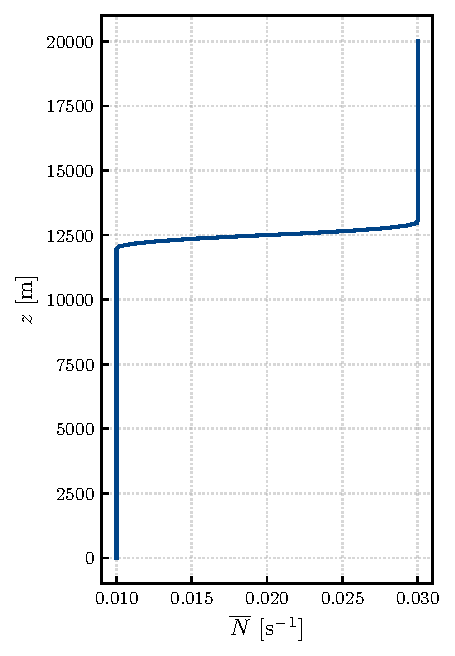
\includegraphics[width=\textwidth]{reference_brunt–väisälä_frequency.pdf}
        \caption{Reference Brunt–Väisälä frequency \eqref{N_bar}}
        \label{fig:N_bar}
    \end{minipage}
    \hfill % Adds flexible space between the two minipages
    \begin{minipage}[t]{0.48\textwidth}
        \centering
        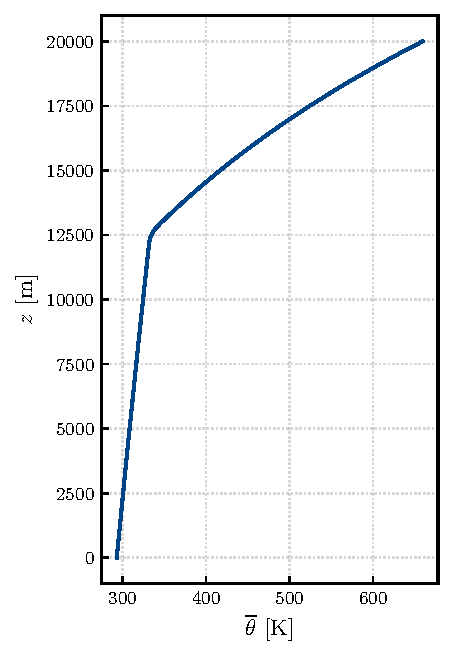
\includegraphics[width=\textwidth]{reference_potential_temperature_profile.pdf}
        \caption{Reference potential temperature profile \eqref{theta_bar}}
        \label{fig:theta_bar}
    \end{minipage}
\end{figure}

We combine the ideal gas law $p = \rho R T$ and the the definition of $\theta$ \eqref{pot_temp} to express the reference density profile:

\begin{equation}\label{rho_bar}
    \overline{\rho}(z) = \frac{\overline{p}}{R \overline{\theta}} \left( \frac{p_s}{\overline{p}}\right)^\kappa
\end{equation}
To determine the pressure profile $\overline{p}(z)$ we use the hydrostatic assumption that $d\overline{p}/dz = -g \overline{\rho}$, substitute in equation \eqref{rho_bar}, and solve the ODE to yield \cite{fehlmann1997pvelements}:

\begin{equation}\label{p_bar}
    \overline{p}(z) = \overline {p}_\text{bot} \left( 1- \frac{\kappa g}{R} \left( \frac{p_s}{\overline{p}_\text{bot}}\right)^\kappa \int_0^z \frac{d \xi}{\overline{\theta}(\xi)}\right)^{1/\kappa}
\end{equation}

\begin{figure}[htbp]
    \centering
    \begin{minipage}[t]{0.48\textwidth}
        \centering
        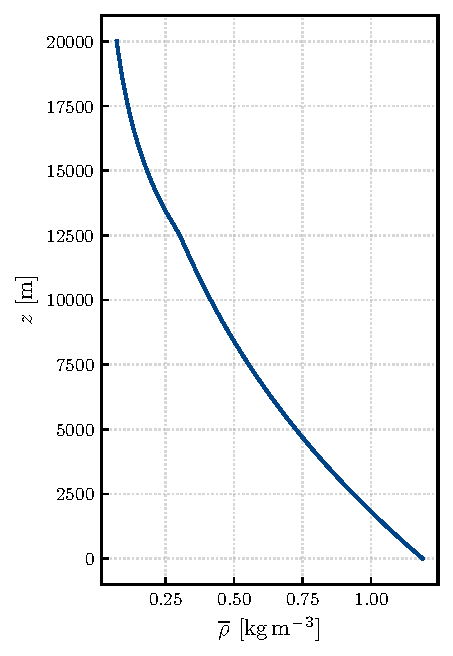
\includegraphics[width=\textwidth]{reference_density_profile.pdf}
        \caption{Reference density profile \eqref{rho_bar}}
        \label{fig:brunt_vaisala}
    \end{minipage}
    \hfill % Adds flexible space between the two minipages
    \begin{minipage}[t]{0.48\textwidth}
        \centering
        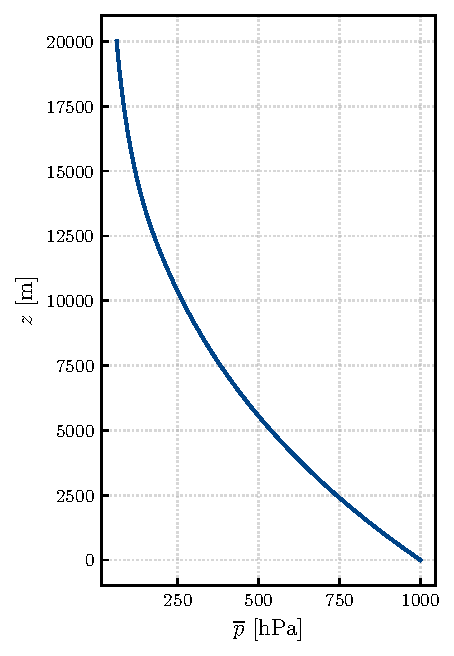
\includegraphics[width=\textwidth]{reference_pressure_profile.pdf}
        \caption{Reference pressure profile \eqref{p_bar}}
        \label{fig:theta_bar}
    \end{minipage}
\end{figure}

\subsection{Boundary Conditions}
To specify the horizontal boundary conditions, we need to choose values of $u$ and $v$. We will define a jet stream aiming to recreate the one shown in \cite{Barnes2022main}. The exact function used is not given, but we can specify a function that also has a maximum magnitude of $u_\text{jet} =\qty{35}{\meter\per\second}$, is centred about the tropopause vertically, is centred about the middle of the domain meridionally, has a Gaussian shape, and has a similar overall size to the one shown in \cite{Barnes2022main} ($y_\text{jet} \approx \qty{500}{\km}$ and $z_\text{jet} \approx \qty{2000}{\meter}$). We will let

\begin{equation}\label{u_boundary}
    u(y,z) = u_\text{jet} \exp\left[ - \left(\frac{y - L_y /2}{y_\text{jet}}\right)^2 - \left(\frac{z - z_\text{trop}}{z_\text{jet}} \right)^2\right]
\end{equation}
\begin{equation}\label{v_boundary}
    v(x,z) = 0
\end{equation}
\begin{figure}[htbp]
    \centering
    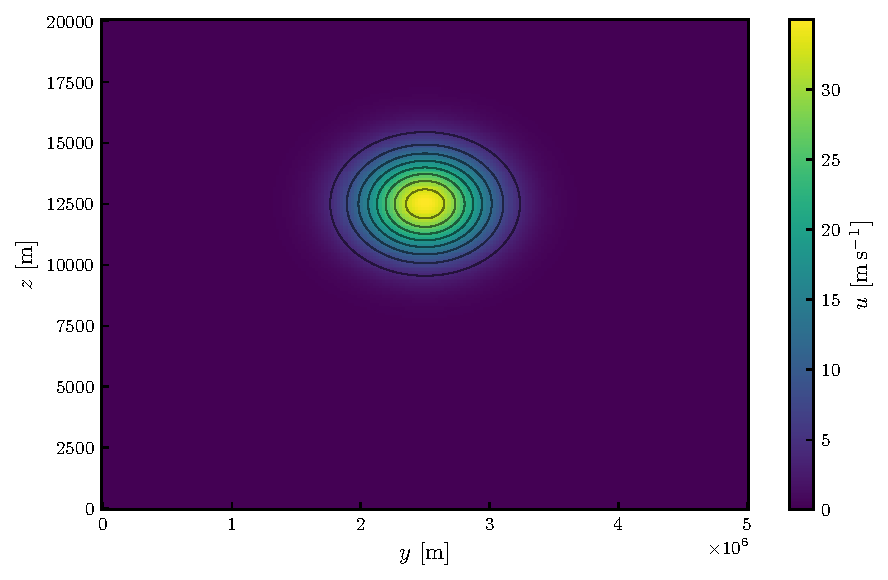
\includegraphics[width=0.96\linewidth]{jet_stream.pdf}
    \caption{Jet stream specified in equation \eqref{u_boundary}}
    \label{fig:jet_stream}
\end{figure}
You may notice that we have not yet defined $\theta^*$. It will be calculated later on to ensure satisfaction of the so-called \textit{Neumann solvability condition}.

\subsection{Source term}
To calculate the source term $q(x,y,z)$

\bibliographystyle{alpha}
\bibliography{sources}

\section{TEMP}
\subsection{Plan}
\begin{enumerate}
    \item Basic structure of the atmosphere
    \item What is potential vorticity?
    \item Introduce Ertel PV
    \item Introduce QG PV
    \item Explain basic derivation of QG PV equation, including splitting into reference and peturbation
    \item What is a stratospheric intrusion and how does it relate to cut off lows
    \item Cut off lows in south africa
    \item Goal of Thesis - initially reproduce barnes work (same BCs), then add timestepping
    \item I.e. investigate the effects of PV anomalies on the weather in an idealised setting
    \item Specify background states and plot them. Explain where necessary
    \item Specify q and plot it
    \item Why we will use finite element and firedrake
    \item Building the mesh and function space in Firedrake
    \item Putting into weak form - why do we multiply by rho?
    \item Solvability condition
    \item Utility functions
    \item Specifying the equation in Firedrake
    \item Choosing solver parameters (matfree vs assembled) - calculate a reasonable ksp rtol and ksp atol - why matrix free is slower (check notebooklm) - why are the coefficients not analytically expressible
    \item Running with MPI
    \item Verify setup is correct using MMS
    \item Calculate time complexity and order of accuracy
    \item Calculating derived quantities such as pressure, velocity and relative vorticity
    \item Reproduction of a few of Barnes' experiments
    \item What happens if we change Brunt-Vaisala to be more realistic
    \item Potentially investigate alternative backgrounds
    \item Feasibility of explicit timestepping - stability condition
\end{enumerate}

\end{document}